\chapter{Minimal problems in computer vision geometry}\labelcha{app}
Many problems from computer vision geometry can be modeled by systems of polynomial equations.
A problem that requires only the minimal subset of data points to solve the problem is called a minimal problem.
A typical example is the 5-point algorithm \cite{5pt} for relative pose estimation between two cameras given five image correspondences only.
In many applications, solvers of these minimal problems are used in the Random Sample Consensus (RANSAC) algorithm \cite{ransac}, where the minimal problems has to be solved repeatedly for a large amount of input data.
Thus, these solvers are required to be fast and efficient.
The state of the art method is to generate these solvers by automatic generators \cite{autogen}, which are based on Gr\"obner basis construction and eigenvectors of multiplication matrices computation.
In these solvers both real and non-real solutions are computed, but the non-real solutions are discarded, since they have no geometric meaning.

In \refsec{POP:sol}, we have proposed and implemented an algorithm, which does not need to compute the superfluous non-real solutions, and therefore may be faster than the standard solvers generated by the automatic generators.
In this section, we compare the speed and numerical stability of the state of the art solvers with our implementations of the moment method algorithm for polynomial system solving.
For this reason, we have selected few minimal problems from computer vision geometry, on which we will compare the selected solvers.

\section{Dataset description}
\input{macros/app_LADIO.tex}
First of all, we describe the scene, which we have chosen for our experiments.
It is a real scene of a sculpture of Buddha head taken for the LADIO \cite{ladio} experiments.
%TODO: cite Ladio experiments
The reconstructed surface of the sculpture can be seen in \reffig{app:LADIO}.
There are \importAppLADIONumCameras{} taken images of the sculpture, from which \importAppLADIONumPoints{} spatial points were reconstructed using a scene reconstruction pipeline including ..., on outliers
%TODO: fill missing part of the pipeline

\begin{figure}[ht]
  \centering
  \begin{subfigure}[b]{0.45\textwidth}
    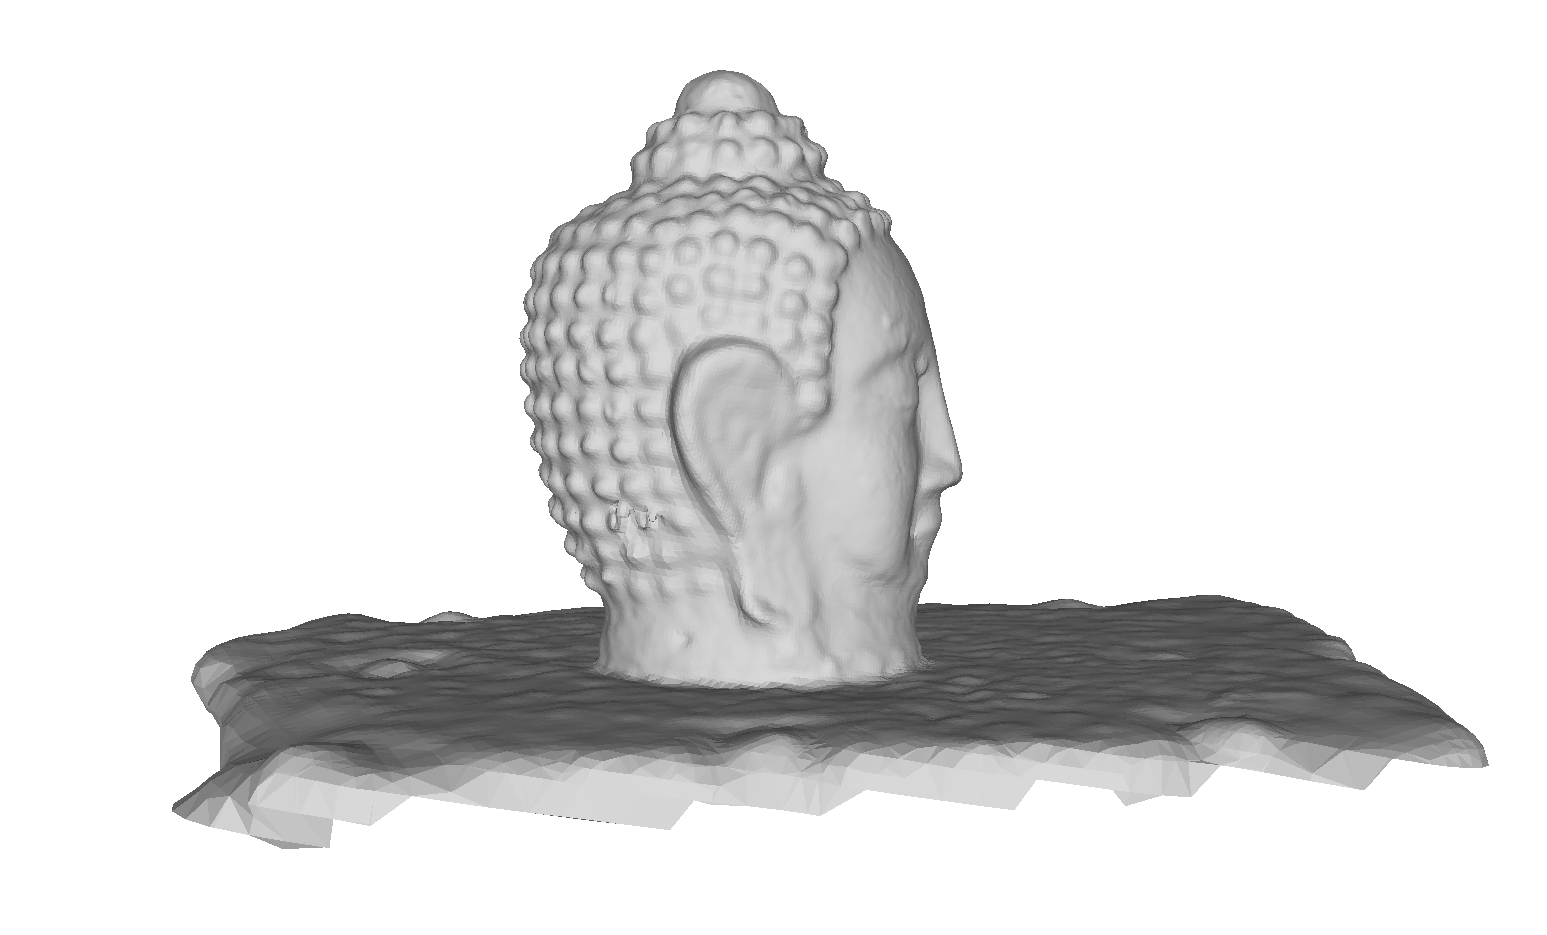
\includegraphics[width=0.95\textwidth]{images/LADIO_01.png}
    \vspace{2mm}
  \end{subfigure}
  ~
  \begin{subfigure}[b]{0.45\textwidth}
    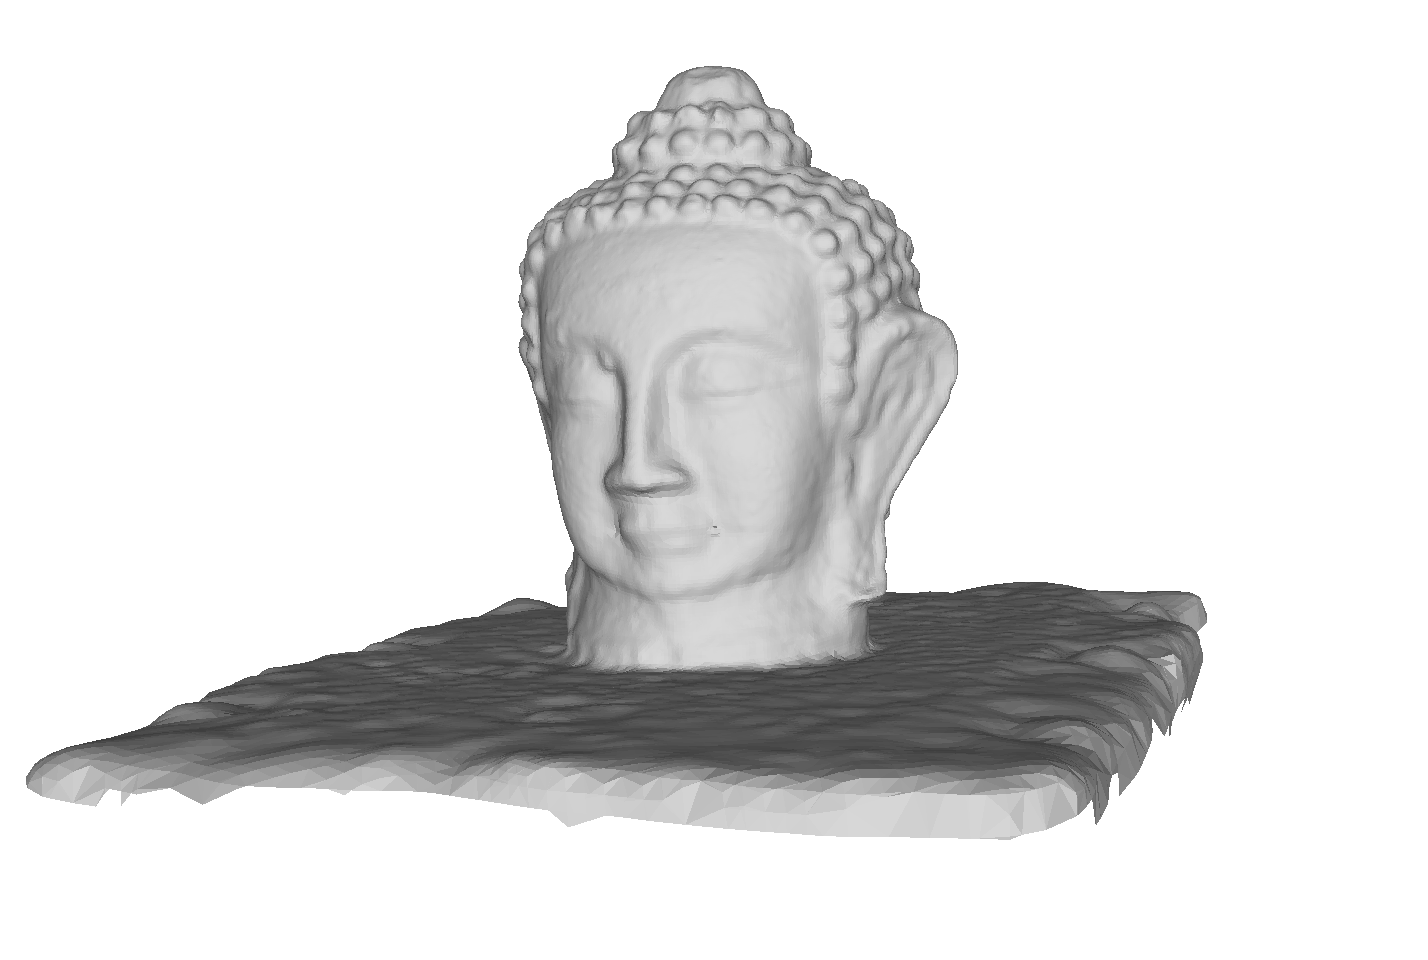
\includegraphics[width=0.90\textwidth]{images/LADIO_02.png}
  \end{subfigure}
  \caption{Sculpture of Buddha head. Surface representing a point cloud reconstructed from the taken images.}
  \labelfig{app:LADIO}
\end{figure}

\section{Calibrated camera pose}
Computation of calibrated camera pose (its rotation and location with respect to the global coordinate system) is one of the typical problems in computer vision.
The pose can be computed from at least three known 3D points and their perspective projection into the image plane, thus the problem is called the perspective-three-point (P3P) problem and it is known since 1841 from \cite{p3p1841}, but its modern and complete description can be found in \cite{P3P}.

\begin{figure}[ht]
  \centering
  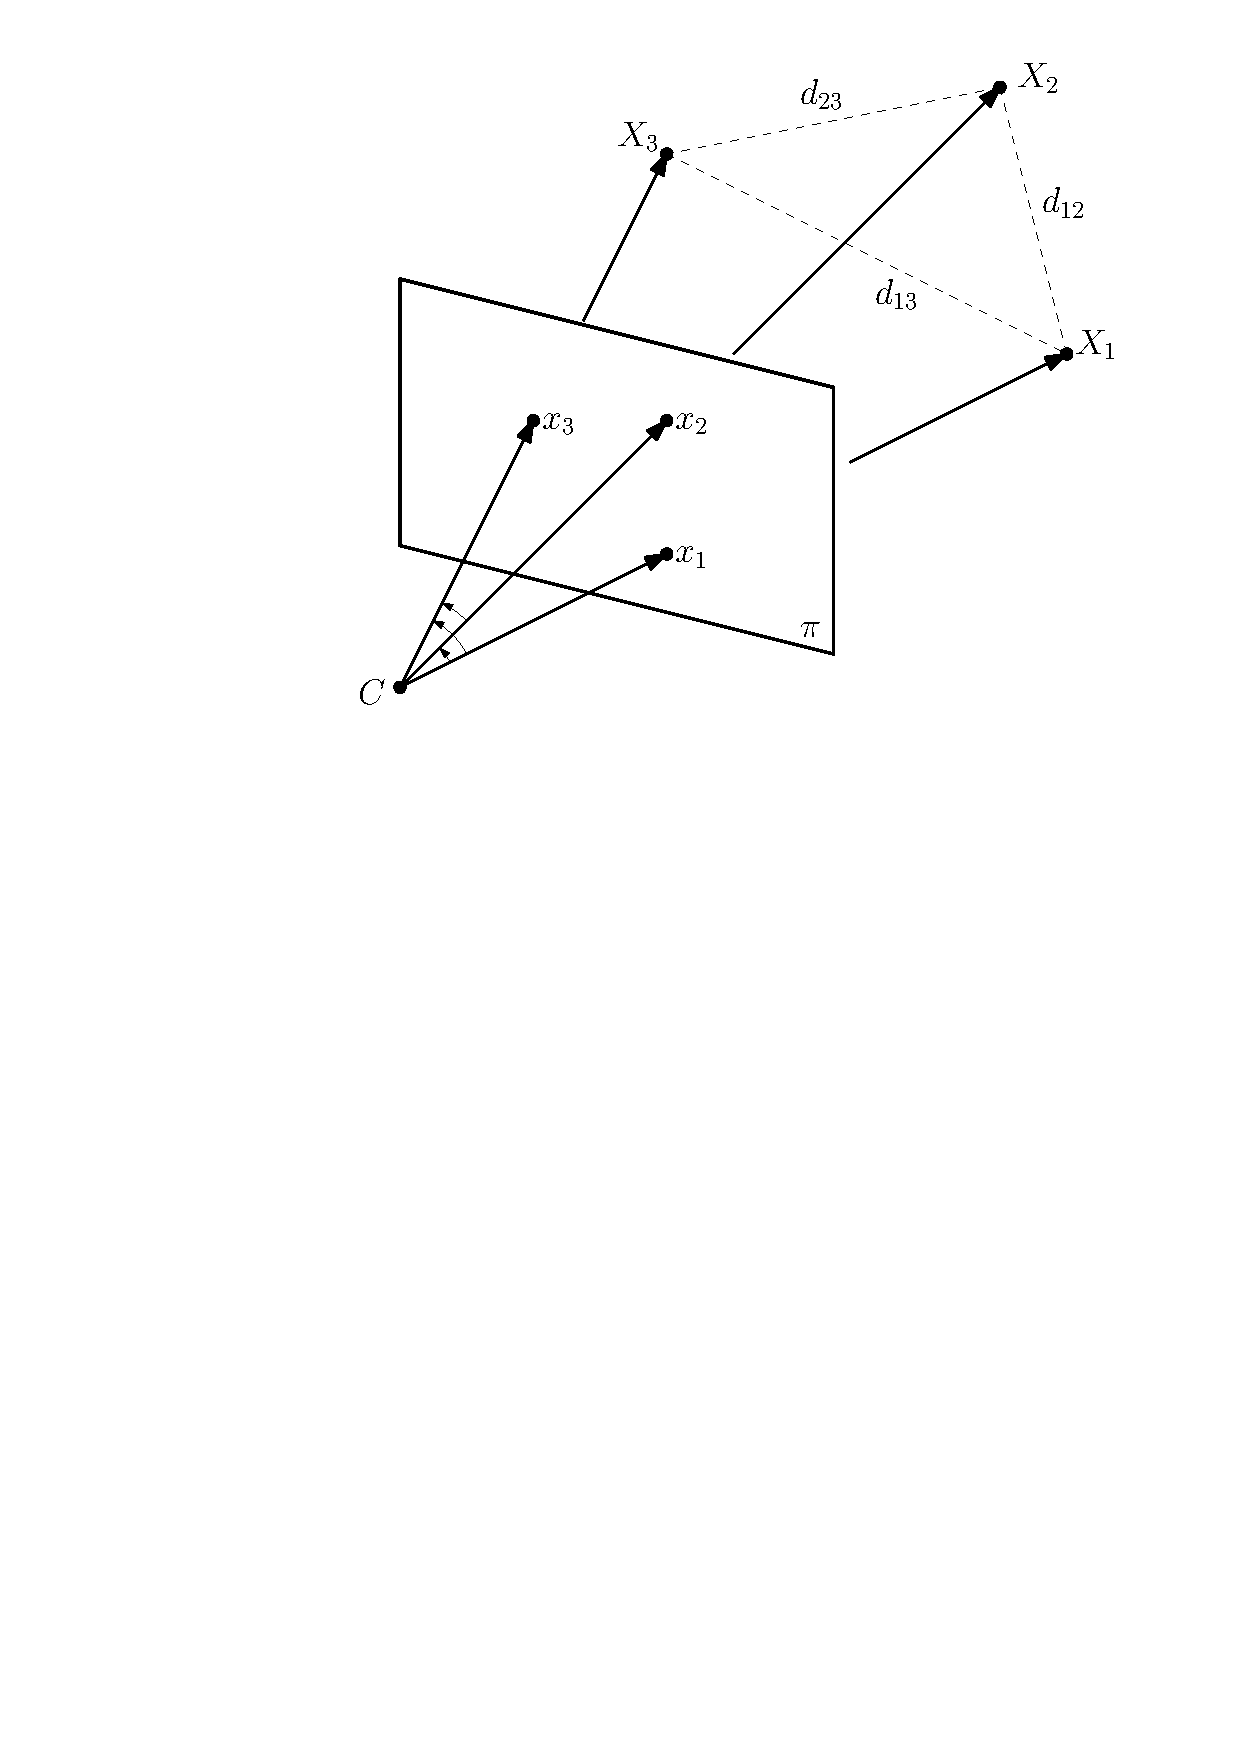
\includegraphics[width=0.5\textwidth]{drawings/P3P.pdf}
  \caption{Scheme of the P3P problem. A pose of a calibrated camera can be computed from three known 3D points $X_1$, $X_2$, $X_3$ and their projections $x_1$, $x_2$, $x_3$ into the image plane $\pi$. The camera projection center is denoted as $C$. Distances $d_{12}$, $d_{23}$, $d_{13}$ denote the distances between the respective 3D points.}
  \labelfig{app:P3P}
\end{figure}

The problem is stated followingly:
Given three 3D points $X_1, X_2, X_3 \in\R^3$ in the global coordinate system and their projections $x_1, x_2, x_3 \in\R^2$ respectively into the image plane in the image coordinate system, we are looking for a camera projection center position $C\in\R^3$ and a camera rotation matrix $R\in\SO$ -- all rotations in 3D space around the origin, such that the projection equation
\begin{align}
  \lambda_i\bmB x_i\\1\bmE &= K\bmB R & -RC\bmE\bmB X_i\\1\bmE
\end{align}
holds for $i=1,2,3$ and $\lambda_i\in\R/\{0\}$, where $K\in\R^{3\times3}$ is known calibration matrix of the camera.
The situation is depicted in \reffig{app:P3P}.

It has been shown that for a general case this problem can be solved by finding roots of a quartic equation in variable $\xi\in\R$
\begin{align}
  a_4\xi^4 + a_3\xi^3 + a_2\xi^2 + a_1\xi + a_0 &= 0\labeleq{app:P3P:4}
\end{align}
with coefficients $a_0, \ldots, a_4\in\R$, which can be computed by the formulae below.
\begin{align}
  a_4 &= -4d_{23}^4d_{12}^2d_{13}^2c_{23}^2+d_{23}^8-2d_{23}^6d_{12}^2-2d_{23}^6d_{13}^2+d_{23}^4d_{12}^4+2d_{23}^4d_{12}^2d_{13}^2+d_{23}^4d_{13}^4\\
  a_3 &= 8d_{23}^4d_{12}^2d_{13}^2c_{12}c_{23}^2+4d_{23}^6d_{12}^2c_{13}c_{23}-4d_{23}^4d_{12}^4c_{13}c_{23}+4d_{23}^4d_{12}^2d_{13}^2c_{13}c_{23}\\
      &-4d_{23}^8c_{12}+4d_{23}^6d_{12}^2c_{12}+8d_{23}^6d_{13}^2c_{12}-4d_{23}^4d_{12}^2d_{13}^2c_{12}-4d_{23}^4d_{13}^4c_{12}\nonumber\\
  a_2 &= -8d_{23}^6d_{12}^2c_{13}c_{12}c_{23}-8d_{23}^4d_{12}^2d_{13}^2c_{13}c_{12}c_{23}+4d_{23}^8c_{12}^2-4d_{23}^6d_{12}^2c_{13}^2\\
      &-8d_{23}^6d_{13}^2c_{12}^2+4d_{23}^4d_{12}^4c_{13}^2+4d_{23}^4d_{12}^4c_{23}^2-4d_{23}^4d_{12}^2d_{13}^2c_{23}^2+4d_{23}^4d_{13}^4c_{12}^2+2d_{23}^8\nonumber\\
      &-4d_{23}^6d_{13}^2-2d_{23}^4d_{12}^4+2d_{23}^4d_{13}^4\nonumber\\
  a_1 &= 8d_{23}^6d_{12}^2c_{13}^2c_{12}+4d_{23}^6d_{12}^2c_{13}c_{23}-4d_{23}^4d_{12}^4c_{13}c_{23}+4d_{23}^4d_{12}^2d_{13}^2c_{13}c_{23}-4d_{23}^8c_{12}\\
      &-4d_{23}^6d_{12}^2c_{12}+8d_{23}^6d_{13}^2c_{12}+4d_{23}^4d_{12}^2d_{13}^2c_{12}-4d_{23}^4d_{13}^4c_{12}\nonumber\\
  a_0 &= -4d_{23}^6d_{12}^2c_{13}^2+d_{23}^8-2d_{23}^4d_{12}^2d_{13}^2+2d_{23}^6d_{12}^2+d_{23}^4d_{13}^4+d_{23}^4d_{12}^4-2d_{23}^6d_{13}^2
\end{align}
Where the distances $d_{12}$, $d_{23}$ and $d_{13}$ are
\begin{align}
  d_{12} &= \|X_1 - X_2\|,\\
  d_{23} &= \|X_2 - X_3\|,\\
  d_{13} &= \|X_1 - X_3\|
\end{align}
and the coefficients $c_{12}$, $c_{23}$ and $c_{13}$ are cosines of angles between respective projection rays, and they can be directly computed from the projected points coordinates.
\begin{align}
  c_{12} &= \frac{x_1^\top K^{-\top} K^{-1}x_2}{\|K^{-1}x_1\|\|K^{-1}x_2\|}\\
  c_{23} &= \frac{x_2^\top K^{-\top} K^{-1}x_3}{\|K^{-1}x_2\|\|K^{-1}x_3\|}\\
  c_{13} &= \frac{x_1^\top K^{-\top} K^{-1}x_3}{\|K^{-1}x_1\|\|K^{-1}x_3\|}
\end{align}

The equation \refeqb{app:P3P:4} may have zero, two or four real roots, but some of them are discarded by checking three polynomial equations, that the law of cosines holds up to some numerical precision in triangles $\triangle\big(CX_iX_j\big)$ for $i,j=1,2,3$ and $i\neq j$, i.e.
\begin{align}
  d_{12}^2 &= \|X_1-C\|^2 + \|X_2-C\|^2 - 2c_{12}\|X_1-C\|\|X_2-C\|,\\
  d_{23}^2 &= \|X_2-C\|^2 + \|X_3-C\|^2 - 2c_{23}\|X_2-C\|\|X_3-C\|,\\
  d_{13}^2 &= \|X_1-C\|^2 + \|X_3-C\|^2 - 2c_{13}\|X_1-C\|\|X_3-C\|.
\end{align}
The camera pose ($C$ and $R$) is then computed from each of the remaining solutions.

The P3P problem is probably the simplest problem, which could be chosen from the computer vision geometry for comparison of the polynomial systems solvers, since only one polynomial of degree four in one variable is given.

\input{macros/app_P3P.tex}
In the experiment, we have randomly selected \importAppPPPNumCameras{} cameras, for each of them \importAppPPPNumPoints{} triplets of 2D--to--3D correspondences has been randomly chosen.
For each triplet, the coefficients $a_0, a_1, a_2, a_3, a_4$ of the equation \refeqb{app:P3P:4} has been precomputed.
Then the real roots $\xi$  of the equation \refeqb{app:P3P:4} has been found by the selected polynomial solvers.
From $\xi$ the camera location $C$ and rotation $R$ has been computed in a standard way.
Then the best tuple $C$ and $R$ minimizing the maximal reprojection error on all correspondences in the image for each camera and solver has been selected.

\subsection{Performance of the polynomial solvers}
We used the described P3P minimal problem to compare following polynomial systems solvers.
Firstly, we would like to see the performance of some state of the art purely algebraic solver.
A possible candidate is a solver generated by the automatic generator \cite{autogen}, which in case of one degree four polynomial equation in one variable is reduced to eigenvectors computation of multiplication matrix of size $4\times4$.
Secondly, the implementation of the moment method from the Polyopt package has been tested.
Thirdly, to be able to compare different implementations of the moment method with different implementation of the SDP solver, we have run the MATLAB implementation with MOSEK toolbox as described in \refsec{POP:sol:impl}.
Lastly, the MATLAB toolbox Gloptipoly \cite{gloptipoly} was used to compare the solvers with another method with built-in optimization.

The histograms of the maximal reprojection errors for the selected tuples of $C$ and $R$ for each polynomial solver can be seen in \reffig{app:P3P:histErr}.
For each estimated camera center position $C$ we have computed the error $e_C$ of the camera position compared to the ground truth values
\begin{align}
  e_C &= \|C-C_{GT}\|,
\end{align}
i.e.\ the distance of the estimated camera position to the ground truth position.
The histograms of these position errors for each polynomial solver are in \reffig{app:P3P:histCDist}.
For each estimated camera rotation $R$ we have computed the residual rotation to the ground truth camera rotation and computed the angle $e_R$ of this residual rotation as
\begin{align}
  e_R &= \arccos\bigg(\frac{1}{2}\Big(\tr\!\big(R_{GT}^{-1}R\big)-1\Big)\!\bigg).
\end{align}
The histograms of the angles of residual rotations for each polynomial solver are in \reffig{app:P3P:histRAngle}.
We have also measured the execution time required to solve each instance of the equation \refeqb{app:P3P:4} by each polynomial solver and histogram of these times can be found in \reffig{app:P3P:histTimes}.

\begin{figure}[ht]
  \centering
  \resizebox{0.95\textwidth}{!}{\input{graphs/app_P3P_err}}
  \caption{Histogram of the maximal reprojection errors of all correspondences in the image for the best camera positions and rotations estimated by the selected polynomial solvers for the P3P problem compared to the maximal reprojection errors computed for the ground truth camera positions and rotations.}
  \labelfig{app:P3P:histErr}
\end{figure}

\begin{figure}[ht]
  \centering
  \resizebox{0.95\textwidth}{!}{\input{graphs/app_P3P_cdist}}
  \caption{Histogram of the errors in estimated camera positions computed by the selected polynomial solvers for the P3P problem with respect to the ground truth camera positions.}
  \labelfig{app:P3P:histCDist}
\end{figure}

\begin{figure}[ht]
  \centering
  \resizebox{0.95\textwidth}{!}{\input{graphs/app_P3P_rangle}}
  \caption{Histogram of the errors in rotation angles computed by the selected polynomial solvers for the P3P problem with respect to the ground truth camera rotations.}
  \labelfig{app:P3P:histRAngle}
  %TODO: what about arccos(>1)
\end{figure}

\begin{figure}[ht]
  \centering
  \resizebox{0.95\textwidth}{!}{\input{graphs/app_P3P_times}}
  \caption{Histogram of the execution times required to compute the P3P problem by the selected polynomial solvers.}
  \labelfig{app:P3P:histTimes}
\end{figure}

Further off, we are interested in the number of real solutions found by the polynomial solvers.
Since the algebraic solver computes all complex solutions first and then the non-real filters out, we are sure that this solver finds all real solutions.
On the other hand, given our observation, the methods based on optimization do not recover all real solutions, despite the theory.
The implementation from the Polyopt package has some numerical issues, which we were unable to remove in the time of writing this thesis, and therefore there is a small chance that the SDP solver fails in its computation and the solution is not found.
Moreover, the number of real solutions is related to the rank of the moment matrix found by the SDP solver, which  numerically depend on how good representative of the set $\K$ we have obtained.
This issue is common for both Polyopt implementation and the MATLAB and MOSEK implementation.
In the case of the Gloptipoly toolbox, which in the first case a polynomial optimization toolbox and not a polynomial system solver, the relaxation order has to be given in advance.
If the relaxation order is not high enough, no solution is found without distinguishing the cases when there is no solution or just the relaxation order is not high enough.
Surprisingly, when the relaxation order is too high, there are not found all the real solutions (e.g.\ only one solution or none is found), because of reasons not known to us.
But since these solvers are typically used in RANSAC-like \cite{ransac} algorithms, it may not be a big issue, when some of the real solutions are not found, of course depending the application.
For the reasons stated above we present in \reftab{app:P3P:numSol} number of all complex solutions and number of real solutions found by each of the polynomial solvers.

\begin{table}[ht]
  \centering
  \input{tables/app_P3P_numberSolutions.tex}
  \caption{Table of numbers of all real and complex solutions and of numbers of found real solutions by each of the polynomial solver for the P3P problem.}
  \labeltab{app:P3P:numSol}
\end{table}

We can see that for the P3P problem there is about $40$ \% of non-real solutions, which need not be computed.
We observe that in practice the moment method based implementations do not found all of the real solutions.
The Polyopt implementation found only $80$ \% of the solutions, but we belive that this can be improved up to $90$ \% success rate, which shows the MATLAB implementation.
Very poor results performed the Gloptipoly toolbox, but they can be probably improved by correct setting of the relaxation order.
On the other hand, from the histograms in Figures \reffignum{app:P3P:histErr}, \reffignum{app:P3P:histCDist}, \reffignum{app:P3P:histRAngle} we can see that the overall results for the P3P problem of the Polyopt implementation and the MATLAB implementation are comparable to the purely algebraic solver, despite they did not find all the real solutions.
Regarding the computation times showed in \reffig{app:P3P:histTimes}, we see that the moment method based implementations are significantly slower than the  pure algebraic solver.
The best results from the moment method based solvers shows the Gloptipoly \cite{gloptipoly} toolbox, but note that we have set the relaxation order in advance, and therefore only one semidefinite program has to be solved for each instance.
